\ifsvnmulti
\svnkwsave{$RepoFile: siminos/chao/KS.tex $}
\svnidlong {$HeadURL$}
{$LastChangedDate$}
{$LastChangedRevision$} {$LastChangedBy$}
\svnid{$Id$}
\fi


\chapter{\KSe}
\label{chap:KS}

\begin{description}

\item[2011-08-24 PC to Chao]
I have created this chapter to help you get started with your own \KS\
notes - edit this your own way as you learn this stuff. You do not
need to reinvent the wheel - clip freely laTeX from Siminos papers
which are all included in this repository.

Keep it up-to-date - if all goes well, it can be used in forthcoming
papers and
\HREF{http://www.online-literature.com/wilde/being_earnest/}
{the thesis}. Please use the same notational conventions and
macros, makes life easier later on.

\end{description}

    \PC{first draft is clipped from Cvitanovi{\'c}, Davidchack and
    Siminos\rf{SCD07}, rpo.tex version of 2009-04-10, please rewrite in
    your own words.}
Recent experimental and theoretical advances\rf{science04}
support a dynamical vision of turbulence:
For any finite  spatial resolution,
a turbulent flow follows approximately for a finite time
a pattern belonging to a
{ finite alphabet}
of admissible patterns.
The long term dynamics is
a {walk through the space of these unstable patterns}.
The question is how to characterize and classify such patterns?
Here we follow the seminal Hopf paper\rf{hopf48}, and  visualize
turbulence not as  a sequence of
spatial snapshots in turbulent evolution,
but as a trajectory in an
 $\infty$-$d$ \statesp\ in which an
instant in turbulent evolution is
a {unique} point. In the dynamical systems approach,
theory of turbulence for a given system, with given boundary conditions,
is given by
(a) the geometry of the \statesp\ and (b) the associated natural measure,
\ie,
the likelihood that asymptotic dynamics visits a given \statesp\ region.

We pursue this program in context of the \KS\ (KS) equation,
one of the simplest physically interesting spatially extended
nonlinear systems.  Holmes, Lumley and Berkooz\rf{Holmes96} offer a
delightful discussion of why this system deserves study as a staging
ground for studying turbulence in full-fledged Navier-Stokes
boundary shear flows.

{
Flows described by partial differential equations (PDEs) are
said to be infinite dimensional because if one writes them
down as a set of ordinary differential equations (ODEs), a set
of infinitely many ODEs is needed to represent the dynamics
of one PDE. Even though their {\statesp} is thus
$\infty$-dimensional, the long-\-time dynamics of viscous
flows, such as Navier-Stokes, and PDEs modeling them, such as
\KS, exhibits, when dissipation is high and
the system spatial extent small, apparent `low-dimensional'
dynamical behaviors. For some of these the asymptotic
dynamics is known to be confined to a finite-\-dimensional
{\em inertial manifold}, though the rigorous upper bounds on
this dimension are not of much use in the practice.

For large spatial extent the complexity of the spatial
motions also needs to be taken into account. The systems
whose spatial correlations decay sufficiently fast, and the
attractor dimension and number of positive Lyapunov exponents
diverges with system size are said\rf{HNZks86,man90b,cross93}
to be extensive, `spatio-temporally chaotic' or `weakly
turbulent.' Conversely, for small system sizes the accurate
description might require a large set\rf{GHCW07} of coupled
ODEs, but dynamics can still be `low-dimensional' in the
sense that it is characterized with one or a few positive
Lyapunov exponents. There is no wide range of scales
involved, nor decay of spatial correlations, and the system
is in this sense only `chaotic.'

For a subset of physicists and mathematicians who study
idealized `fully developed,' `homogenous' turbulence the
generally accepted usage is that the `turbulent' fluid is
characterized by a range of scales and an energy cascade
describable by statistic assumptions\rf{frisch}. What experimentalists,
engineers, geophysicists, astrophysicists actually observe
looks nothing like a `fully developed turbulence.' In the
physically driven wall-bounded shear flows, the turbulence is
dominated by unstable \emph{coherent structures}, that is,
localized recurrent vortices, rolls, streaks and like. The
statistical assumptions fail, and a dynamical systems
description from first principles is called for\rf{Holmes96}.
} %end

Dynamical \statesp\ representation of a PDE is
$\infty$-dimensional, but the KS flow is strongly contracting
and its non-wondering set, and, within it, the set of
invariant solutions investigated here, is embedded into a
finite-dimensional inertial manifold\rf{FNSTks85} in a
non-trivial, nonlinear way. `Geometry' in the title of this
paper refers to our attempt to systematically triangulate
this set in terms of dynamically invariant solutions (\eqva,
\po s, $\ldots$) and their unstable manifolds, in a PDE
representation and numerical simulation algorithm independent
way. The goal is to describe a given `turbulent' flow
quantitatively, not model it qualitatively by a
low-dimensional model. For the case investigated here, the
\statesp\ representation dimension $d \sim 10^2$ is set by
requiring that the exact invariant solutions that we compute
are accurate to $\sim 10^{-5}$.

{
Here comes our quandary. If we ban the words `turbulence' and
`spatiotemporal chaos' from our study of small extent
systems, the relevance of what we do to larger systems is
obscured. The exact unstable coherent structures we determine
pertain not only to the spatially small `chaotic' systems,
but also the spatially large `spatiotemporally chaotic' and
the spatially very large `turbulent' systems.
So, for the lack of more precise nomenclature, we take the
liberty of using the terms `chaos,' `spatiotemporal chaos,'
and `turbulence' interchangeably.
} %end


In previous work, the \statesp\ geometry and the natural measure for
this system have been
studied\rf{Christiansen97,LanThesis,lanCvit07} in terms of unstable
periodic solutions restricted to the antisymmetric subspace of the
KS dynamics.

The focus in this paper is on the role continuous symmetries
play in spatiotemporal dynamics. The notion of exact
periodicity in time is replaced by the notion of relative
spatiotemporal periodicity, and \reqva\ and \rpo s here play
the role the \eqva\ and \po s played in the earlier studies.
Our search for \rpo s in KS system was inspired by Vanessa
L{\'o}pez\rf{lop05rel} investigation of {\rpo s} of the
Complex Ginzburg-Landau equation.  However, there is a vast
literature on {\rpo s} since their first appearance, in
Poincar\'e study of the 3-body problem\rf{ChencinerLink,rtb},
where the Lagrange points are the \reqva.  They arise in
dynamics of systems with continuous symmetries, such as
motions of rigid bodies, gravitational $N$-body problems,
molecules and nonlinear waves. Recently Viswanath\rf{Visw07b}
has found both \reqva\ and \rpo s in
the plane Couette problem.
    {
A Hopf bifurcation of a traveling
wave\rf{AGHO288,AGHks89,Krupa90} induces a small
time-dependent modulation. Brown and Kevrekidis\rf{BrKevr96}
study bifurcation branches of \po s and \rpo s in KS system
in great detail. For our system size ($\alpha=49.04$ in their
notation) they identify a \po\  branch. In this
context \rpo s are referred to as `modulated traveling
waves.' For fully chaotic flows we find this notion too
narrow. We compute 60,000 \po s and \rpo s that are in no
sense small `modulations' of other solutions, hence our
preference for the well established notion of a `\rpo.'
          }

Building upon the pioneering work of
\refrefs{KNSks90,ksgreene88,BrKevr96}, we undertake here a
study of the \KS\ dynamics for a specific system size $L =
22$, sufficiently large to exhibit many of the features
typical of `turbulent' dynamics observed in large KS systems,
but small enough to lend itself to a detailed exploration of
the  \eqva\ and \reqva, their stable/unstable manifolds,
determination of a large number of \rpo s, and a preliminary
exploration of the relation between the observed
spatiotemporal `turbulent' patterns and the \rpo s.

In presence of a continuous symmetry any solution belongs to a group
manifold of equivalent solutions. The problem: If one is to
generalize the \po\  theory to this setting, one needs to
understand what is meant by solutions being nearby (shadowing) when
each solution belongs to a manifold of equivalent solutions. {In a
forthcoming publication\rf{SCD09b} we resolve this puzzle by implementing
symmetry reduction.} Here we demonstrate that, {for \rpo s visiting the
neighborhood of equilibria,} if one picks any
particular solution, the universe of all other solutions is rigidly
fixed through a web of heteroclinic connections between them. This
insight garnered from study of a 1-dimensional \KS\ PDE is more
remarkable still when applied to the plane Couette flow\rf{GHCW07},
with 3-$d$ velocity fields and two translational symmetries.

The main results presented here are: [NONE AS YET]

\section{\KSe\ - a review}
\label{chap:KSreview}

\begin{description}

\item[2011-08-24 PC to Chao]
Please keep writing and rewriting in this section the draft of the
\KSe\ review to eventually include in your thesis.

Read also Siminos blog section \emph{ \KS: literature survey}, you might
want to copy some of that stuff into your review of this section. Other
useful sources are Lan thesis\rf{LanThesis} and Siminos
thesis\rf{SiminosThesis}.

\end{description}



\section{Reading}
\label{s:KSreading}

\subsection{Spatiotemporal chaos in terms of unstable recurrent patterns}
\label{s:Christiansen97}

\begin{description}

\item[2011-08-24 Chao]
The central work of using unstable recurrent patterns describing
spatiotemporal chaos is the search of \po s, especially unstable \po s.
Stable ones are not as important because they are attractive, within
their respective basins of attraction, and display no chaotic behavior.
The unstable ones are typically \emph{saddles}, with both unstable and
stable eigendirections. In the unstable directions, they shoot out
neighboring points while in the stable directions they draw them in. Thus
dynamics is called ``hyperbolic'' because its linearized behavior is
hyperbolic. Taken together, the set of unstable \po s is the source of
chaotic behavior. While we cannot find \emph{all} unstable \po s of a
system (their number is infinite, growing exponentially with the period
of the orbit), we can decompose its dynamics as the combination of
influences of the near \po s.

This paper consists of 5 parts. I mainly focused on the 4th part:
one-dimensional visualization, which illustrate in detail how we find
\po\  and visulize them in low dimensions.

Here is my understanding of the whole process: First we choose a
\PoincSec\ in the full \statesp\ and let the dynamical system evolve for
a sufficiently long time to give us enough points on the section. This
enables us to define a return map for the section. Within the section,
iterating the map itself may generate discrete-time \po s, which can be
found out exhaustively (in finite resolution) by utilizing symbolic
dynamics. Before we use symbolic dynamics, we have to build an intrinsic
arclength coordinate system; for the parameter values studied here, close
to onset of chaos, this return map is approximately unimodal. This
situation is very special, due to only one direction of any \po\ being
unstable. The remaining ones (except for the single marginal eigenvalue
due to Since periodic points in a discrete time \po\ belong to a
continuous \po\  in the full \statesp\, we can integrate from these
periodic points to recover the full space \po.

Here are some detailed questions:

In the third paragraph of part 4, it is said
``The $i$th cycle point  $s_i$ is mapped onto its image $s_{\sigma i} = f(s_i)$ where $\sigma i$ denotes  the label of the next periodic point in the cycle.''


So that means $\sigma i$ is not meant to be $i+1$, right? Because the order of different cycle points is given in following way: ``there exists a fixed point which
is not connected to the attractor (the point
$\overline{0}$ in \reffig{returnmap}) - we
choose this fixed point
as the starting point and assign it number $1$.
Point number $2$ is the periodic point in the sample
which is closest (in the full space)
to this fixed point, and the $n$-th point is determined as the point
which has the minimum distance from the point number $n-1$ among
all the periodic points which have not yet been enumerated.
Proceeding this way, we order all the periodic points that we have found
so far.''

So from this we could know that the order of periodic points on the
section is not the order of time evolution of these points. Right? But if
it is true, that seems to contradict with the illustration under figure
4?

\item[2011-08-30 Predrag]
For a general orbit we  label points in map iteration by
\beq
s_{n+1} = f(s_n)
\ee{curvTime}
where $n=\{1,2,\cdots\}$ is the discrete time.
For a periodic orbit of period $n$ we use $s_a$
where $a = \Ssym{1}\Ssym{2}\cdots\Ssym{n}$, and the
dynamics acts on the label as a cyclic permutation,
$\sigma s_a = \Ssym{2}\cdots\Ssym{n}\Ssym{1}$
\beq
s_{\Ssym{2}\cdots\Ssym{n}\Ssym{1}} =
    f(s_{\Ssym{1}\Ssym{2}\cdots\Ssym{n}})
\,,
\ee{curvPO}
where the block $\Ssym{1}\Ssym{2}\cdots\Ssym{n}$ is the cycle itinerary.
For example, 11100-cycle point $s_{11100}$ is mapped into next cycle
point $s_{11001}$ which can be far away; spatial ordering of cycle points
is given by alternating binary trees and such...

Unfortunately, in this application we discretize the 1-dimensional
unstable manifold, so there is yet another integer suffix which refers to
a spatially ordered set of points, such that
\beq
s_{j-1} < s_{j} < s_{j+1}
\,.
\ee{curvPO}

Can you try to add text to ChaosBook.org
smale.tex, section {\em Parametrization of invariant manifolds}
which clarifies this for the next reader? Maybe a drawing with
a 3-cycle would be helpful. Not sure

[will continue this later]


\item[2011-08-24 Chao]
A prerequisite question is that from paragraph 2 to paragraph 3, the
phrase``periodic points'' should mean the points on the reduced
1-dimensional map, right?(or points on the N-1 dimensional Poincare
section?) If so, since the reduced 1-dimensional map is a projection from
higher dimension, it could be that two different periodic points have the
same projection? What to do about that?


In figure 1, it is said `` The lower arrow indicates the kink where the
invariant set A starts to overlap with $\theta SA$''. I don't understand
how the overlap of A and $\theta SA$ is connected to the kink in the
Feigenbaum tree. I can don't have the intuition of how is it like that
``A overlaps with $\theta SA$''. Can you show me some simple examples to
illustrate it pictorially so that I can have an intuitive feeling?

\end{description}

\subsection{Unstable recurrent patterns in {\KS} dynamics}
\label{s:lanCvit07}

%\item[2011-08-24 PC to Chao]
Notes, questions \etc\ while studying Lan and Cvitanovi{\'c}\rf{lanCvit07}.

\begin{description}

\item[2011-09-03 Chao]
Comparing with the previous paper, \refsect{s:Christiansen97}, this paper
investigates a slightly larger \KS\ system which allows for more than one unstable
eigen-direction. I haven't got much more new things than I did in the previous
one because the idea in this paper is the same with the previous one.

\item[2011-09-12 Predrag] You are a harsh judge of men. Lan worked on
this over 6 years, and there is nothing new? That'll teach him to work
harder next time...
                            \toCB

\begin{itemize}
    \item
This slightly larger \KS\ system allows for more than one important \eqv\
solution, and is the first example of partitioning of its $\infty$\dmn\
\statesp\ into several neighborhoods.
    \item
It discusses the \eqv\ of KS on infinite domain, something not even mentioned
in \refref{Christiansen97}.
    \item
It finds an insanely long \emph{stable} \po, embedded in and visually
indistinguishable of the turbulence around it.
    \item
[Chao, fill in other novelties here]
\end{itemize}

\item[2011-09-12 Chao]
Sorry for the improper wording. I meant that I could understand more details in the paper only if I start compute myself such that I can have more insight of the method and difficulties in this problem. Just that I have not got yet, doesn't mean that it dosen't have novelties:)

\item[2011-09-03 Chao]

In page 4, section A, it is said ``We pick any point on a typical orbit
of (4). It corresponds to a loop in 3-d state space of (8) and so can be
used to initialize the search for an u(x) profile periodic on [0,L]''.
So, a point in the Fourier space periodic orbit is mapped into a loop in
real space? Don't feel like this is correct.

For your convenience,

equation (4):
\beq
\displaystyle\dot{a}_{k}
= (k/\tilde{L})^{2}(1-(k/\tilde{L})^{2})a_{k}
- (k/\tilde{L})\sum\nolimits^{+\infty}_{m=-\infty}a_{m}a_{k-m}
\eeq

equation (8)
\beq u_x = v, v_x = w, w_x = u^2 - v -E
\eeq
For the rest part of the paper, I think I can well understand them only
if I start computation myself. I don't even know where to start to ask if
I don't go through the process. So I'll record the question here later if
I have any question in my own computation.
Plus, for further study and better understanding of this paper, I should
read references [22], [33]-[35] in particular.

\end{description}

\subsection{The steady states of the {Kuramoto-Sivashinsky} equation}
\label{s:ksgreene88}

Notes on Greene and Kim\rf{ksgreene88}.

\begin{description}

\item[2011-09-12 PC to Chao]
Search siminos blog for Greene, clip and paste his notes and figures
to here - might be helpful.

\noindent
[ ] {\bf 2011-09-12 Predrag} mark this box once you have entered the
edits and discussed them with me.

\end{description}

\subsection{60,000 \rpo s and no place to go}
\label{s:SCD07}

\begin{description}

\item[2011-08-24 PC to Chao]
Please enter here your notes, questions \etc\ while studying
Cvitanovi{\'c}, Davidchack and Siminos\rf{SCD07},
\emph{On the \statesp\ geometry of the {\KS} flow}

\item[2011-09-03 Chao ]
This paper discussed in detail how symmetry simplifies the search for
equilibria/relative equilibria and peoriodic/relavtive periodic orbits. I
mainly focused on the first half and appendices which describes the idea
and computation methods. The rest of the paper is just details and
results of computation which I can only master by starting computing
myself.

\item[2011-09-12 Predrag]  You are a harsh judge of men. This is a
significant part of Siminos thesis, and it is `just details?'

\item[2011-09-03 Chao]
In appendix A, I checked equation (A.6) and it is correct. But the notion
of writing equation in Fourier transform operator is not so explicit.
That's why at first I was stuck on them. Equation (A.5) is just equation 4.2 in
Chaosbook. Here I rewrite (A.5) and (A.6) as (repeated indices summed over):
\bea
\dot{b}_k &=& \frac{\partial v_k(a)}{\partial a_j}b_j
\continue
v_k(a) &=& \dot{a}_k = (q^2_k - q^4_k)a_k - \frac{iq_k}{2}\sum\nolimits_ma_ma_{k-m}
\continue
\frac{\partial v(a)_k}{\partial a_j} &=&
(q^2_k - q^4_k) - \frac{iq_k}{2}\sum\nolimits_m(\delta_{mj}a_{k-m}+a_m\delta_{j,k-m})
\continue
&=& (q^2_k - q^4_k) - {iq_k}a_{k-j}
\,.
\label{KSstabMat1}
\eea

Combining the last two equations, we obtain:
\beq
\dot{b}_k = (q^2_k - q^4_k)b_k - iq_k\sum\nolimits_ja_{k-j}b_j
\,.
\label{KSstabMat2}
\eeq
The last term is discrete convolution of vector a and b in Fourier space,
which corresponds to component-wise product of two vectors in original
space due to Fourier transform's property. That is why it has the form in
(A.6).

We have to compute vector $\dot{b}_k$ because we have to observe how a
small deviation from the periodic orbit described by ${a_k,\dot{a}_k}$
evolves and integrate segment by segment(e.g. numerical integral) to
obtain Floquet Multipliers and thus obtain Jacobian matrix and Lyapunov
exponents.

Appendix C gives the searching algorithm of relative periodic orbits. I
got the idea, waiting to embark on real computation to knock down more
blockade.

\end{description}

\subsection{Turbulence, coherent structures, dynamical systems and
symmetry}
\label{s:Holmes96}

\begin{description}

\item[2011-08-24 PC to Chao]
Please enter here your notes, questions \etc\ while studying
Holmes, Lumley and Berkooz\rf{Holmes96}.

\end{description}

\section{\KS: literature survey}
\label{sec:KSlit}
% Vaggelis               jan 20 2007


The {1\dmn} \KSe\
as given in \refrefs{ku,siv} is (up to overall scaling factors):
	\PC{moved here from rpo\_ks/}
\beq
    y_t=-y_x^2/2-y_{xxxx}-y_{xx}
\,,\qquad       x \in [0,L]
\,,
    \label{eq:KSeOR}
\eeq
with periodic boundary conditions in the $[0,L]$ interval. The form used
here
\beq
    u_t=uu_x-u_{xxxx}-u_{xx}
\,.
    \label{eq:KSeAP}
\eeq
is obtained from \refeq{eq:KSeOR} by differentiating with respect to $x$
and setting \PCedit{$u=-y_x$}.
In study of {1\dmn} \KS\ \eqva\ $x$ in \refrefs{LanThesis,ksgreene88}
is interpreted as ``time", so $y$ is a height of a front, and $y_x$ its ``velocity".
In the literature  both forms of the equation are
referred to as the \KSe.
% According to \refref{TsveTri89} the solutions of the two equations
% differ considerably despite the simple way they are related.
% \PC{Whatever that means? They are related by a derivative one way,
% integration constant the other. Enter TsveTri89 into siminos.bib}

\paragraph{\Eqva\ according to Greene and Kim:}
%
The form of \KSe\ studied by Greene and Kim\rf{ksgreene88} is
\beq
    y_t=-4y_{xxxx}-\alpha\left(y_{xx}+\frac{1}{2}y_x^2
            -\frac{1}{4\pi}\int_0^{2\pi}y_x^2\ dx\right)
\,,\qquad       x \in [0,2\pi]
\,,
    \label{eq:KSeGreeneKim}
\eeq
with  periodic boundary condition on the interval $[0,2\pi]$.
Mean elastic energy density of a spatial profile $y(x,t)$ is defined by
\beq
    E=\frac{1}{2\pi}\int_0^{2\pi}y_x^2\, dx\,.
    \label{KSenergy}
\eeq
% \ES{This definition does not only apply to equilibria. Greene and
% Kim also study the transfer of energy between modes
% in non-stationary trajectories.}.
Taking the derivative of \refeq{eq:KSeGreeneKim}
with respect to $x$ and substituting $y_x=-u$ leads to
\[
    u_t=4u_{xxxx}+\alpha\left(u_{xx}-uu_x\right)
\,.
\]
Rescaling
\beq
    \tilde{x}=\frac{\sqrt{\alpha}}{2} x
\,,\qquad
    \tilde{t}=\frac{\alpha^2}{4} t
\,,\qquad
    \tilde{u}=\frac{2}{\sqrt{\alpha}} u
    \label{eq:GKscale}
\eeq
brings the Greene-Kim equation to the form \refeq{eq:KSeAP} used here.
The dimensionless system size $\tildeL=L/2\pi$ is related to
the Greene-Kim parameter
through $\tildeL=\sqrt{\alpha}/2$.
The system size $L=22$ studied here corresponds to $\alpha=49.0395$.

The ``kinetic energy'' reads in our units:
\PC{shouldn't there be a prefactor $\frac{1}{2}$?}
\beq
    \tilde{E}=\frac{1}{L}\int_0^{L}\tilde{u}^2\, d\tilde{x}\,.
\eeq
Integrating \refeq{eq:stdks} in $[0,L]$ we get $c=\tilde{E}$,
since the terms involving $u_x$ and $u_{xxx}$ vanish due to periodicity.
\PC{
    Now that you have explained that the integration constant $c$ in
\refeq{eq:stdks} is ``elastic energy" $E$,
please rewrite other sections accordingly. Also try to plot an analogue of
the [wall forcing] vs. [heat dissipation] of plane Couette. On this plot
appropriate integrals of
$(u_{xx}(x,t), u_{xx}(x,t))$ are the
[negative viscosity forcing] vs [hyperviscous damping] axes,
all \eqva\ and \reqva\ are on the diagonal, all \po s and \rpo s
are loops, and a typical turbulent
trajectory has the mean on the diagonal, but visitation frequency might
indicate to us which \eqva\ and \rpo s are the dynamical important ones.
    }
From the scalings \refeq{eq:GKscale} we have $\tilde{E}=\frac{4}{\alpha}E$.


%%%%%%%%%%%%%%%%%%%%%%%%%%%%%%%%%%%%%%%%%%%%%%%%%%%%%%%%%%%%%%%%
\begin{figure} \label{fig:GreeneKim}
\centering
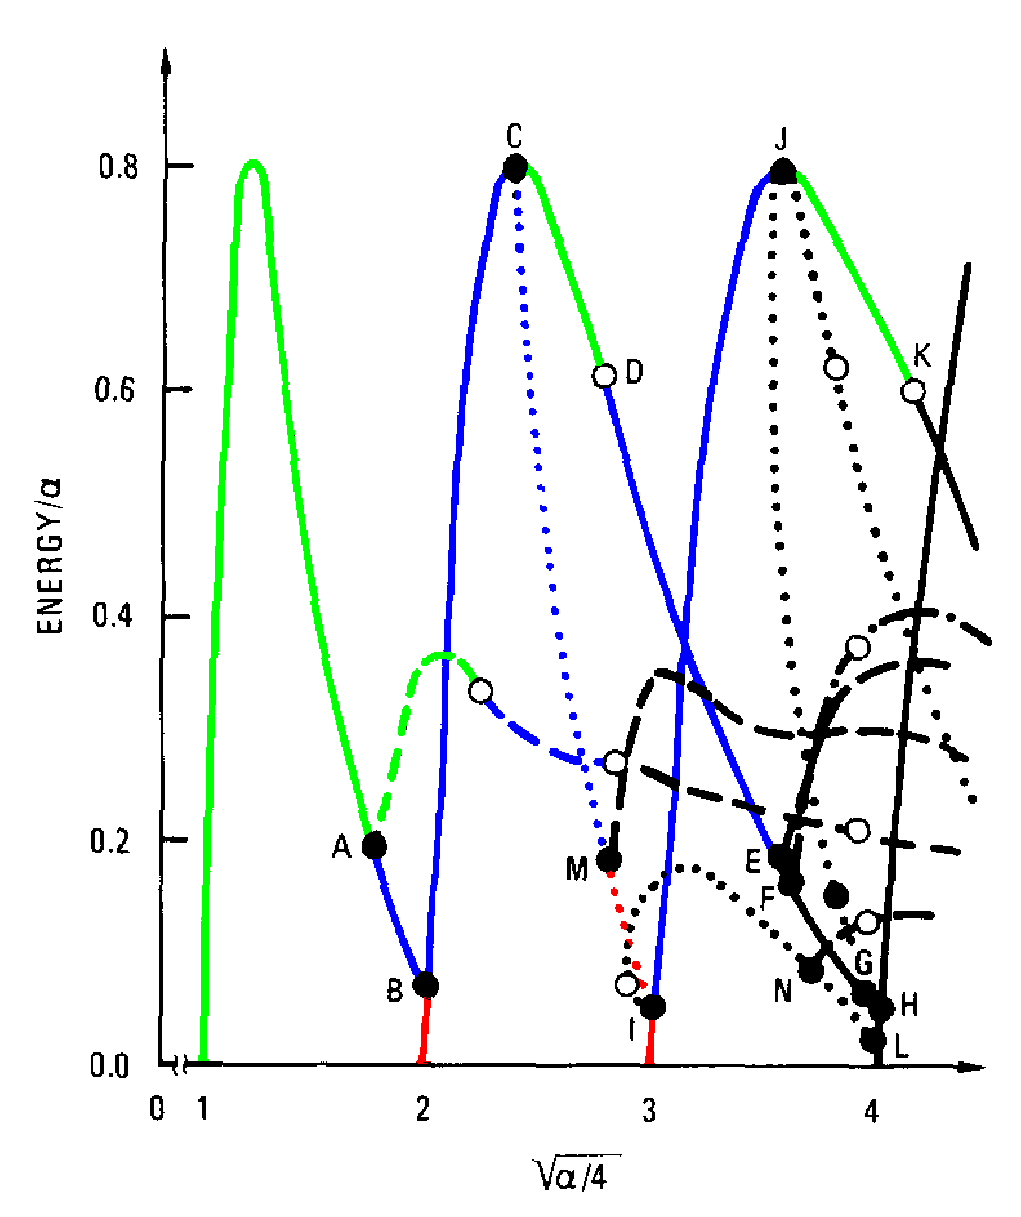
\includegraphics[width=0.5\textwidth]{../rpo_ks/figsUnused/GreeneKimBifColor}
    % \vspace*{-5pt}
\caption[The ``energy'' of \eqva\ as a function of the bifurcation parameter]
        {
The ``energy'' of \eqva\ as a function of the bifurcation
parameter $\tildeL=\sqrt{\alpha}/2$, from \refref{ksgreene88}.
The solid curves denote $N$-cell solutions,
dotted curves GLMRT, the dash-dotted curve the
giant states, and dashed curves the propagating solutions.
Open circles indicate Hopf bifurcations.
We have color-coded the branches to reflect the number of unstable
eigenvalues (or complex pairs). Red: 2 unstable eigenvalues, Blue: 1
unstable eigenvalue, Green: stable. Solutions not
resolved in \refref{ksgreene88} or of no interest
to our present purposes have been left black.
        }
\end{figure}
%%%%%%%%%%%%%%%%%%%%%%%%%%%%%%%%%%%%%%%%%%%%%%%%%%%%%%%%%%%%%%%%%%

Greene and Kim study extends the earlier work\rf{Mks86,laquey74}
on the \KS\ \eqva\ and their bifurcations. The
bifurcation diagram reffig(fig:GreeneKim) summarizes the results
relevant to the system sizes studied here.
\PC{
Please redraw bifurcation diagram reffig(fig:GreeneKim) from the
scratch in xfig (that will make it easier for me to edit), labeling
the axes with our symbols, and various \eqva\ with our - still in flux -
notation for them. Indicate also by circles the nature of
bifurcations for $u(x) = 0$ \eqv. I though those were Hopf? Wrong?
For the thesis, make schematic plots of each bifurcation,
in style of Strogatz or whatever standard textbook on bifurcations
you like the best. You will help Jonathan and me understand what precisely
these bifurcations are. Thanks!
    }
\PC{indicate Christiansen at al. and Lan and Cvitanovi\'c  choices of
    system size on the $\tildeL$ axis
    in reffig(fig:GreeneKim). Might require thinking - they are
    in the antisymmetric subspace, I tend to 1/2 them but here one should
    not.}

For small $\alpha$ the only \eqv\ of the system is the constant solution $y(x,t)=0$,
which is globally attracting
for $\tildeL=\sqrt{\alpha}/2<1$. At $\tildeL=N$, with $N$ integer,
the $N$th harmonic becomes unstable and the constant solution
bifurcates to the so called $N$-cell states.
These states contain only the multiples of the $N$th
harmonic, {\ie} only the components $a_N,a_{2N},...$ in our notation.
Moreover, the $N$-cell states are found to be symmetric (in our case, since $u=y_x$ they will be
antisymmetric).
Greene and Kim show that symmetric solutions are \eqva, not \reqva.
At point $A$ in reffig(fig:GreeneKim) the $1$-cell state loses stability
and bifurcates to a stable,
asymmetric \reqv, which later on becomes unstable through a Hopf bifurcation.
\PC{harmonize our notation with the ``$N$-cell state" notation}

At $\tildeL=2$ the system has become large enough that a $2$-cell \eqv\ appears. At point $B$
in reffig(fig:GreeneKim) the $1$-cell branch merges to the $2$-cell branch. In general each $N$-cell branch merges to the corresponding $2N$-cell branch.

At point $C$ in reffig(fig:GreeneKim) the $2$-cell state
bifurcates to a type of \eqv\ solution found by La Quey,
Mahajan, Rutherford and Tang\rf{laquey74} and generalized by
Greene and Kim who refer to them as GLMRT \eqva. GLMRT
solutions are symmetric ($u(x)$ is antisymmetric) and can be
roughly described as long-wave distorted $N$-cell states.

The last type of solution identified in \refref{ksgreene88} appears at point $F$
in reffig(fig:GreeneKim) and is called a
``giant" state because its amplitude grows as the system size increases.

According to the bifurcation diagram reffig(fig:GreeneKim),
at the point that corresponds to system size $\tildeL=\alpha^{1/2}/2=3.501$
studied here,
the {\eqva} we expect are the $2$- and $3$-cell states ($\EQV{2}$ and $\EQV{3}$ respectivelly), the GLMRT state that bifurcates from a $3$-cell state at point $I$ ($\EQV{1}$),
the \reqva\ that belong to the branches starting at points $A$ ($\REQV{\pm}{1}$),
and $M$ ($\REQV(\pm){2}$).
    \ES{\refeq{fig:ksBifDiag} is preliminary, finalize.}

%%%%%%%%%%%%%%%%%%%%%%%%%%%%%%%%%%%%%%%%%%%%%%%%%%%%%%%%%%%%%%%%
\begin{figure}
\begin{center}
    %RESTORE? 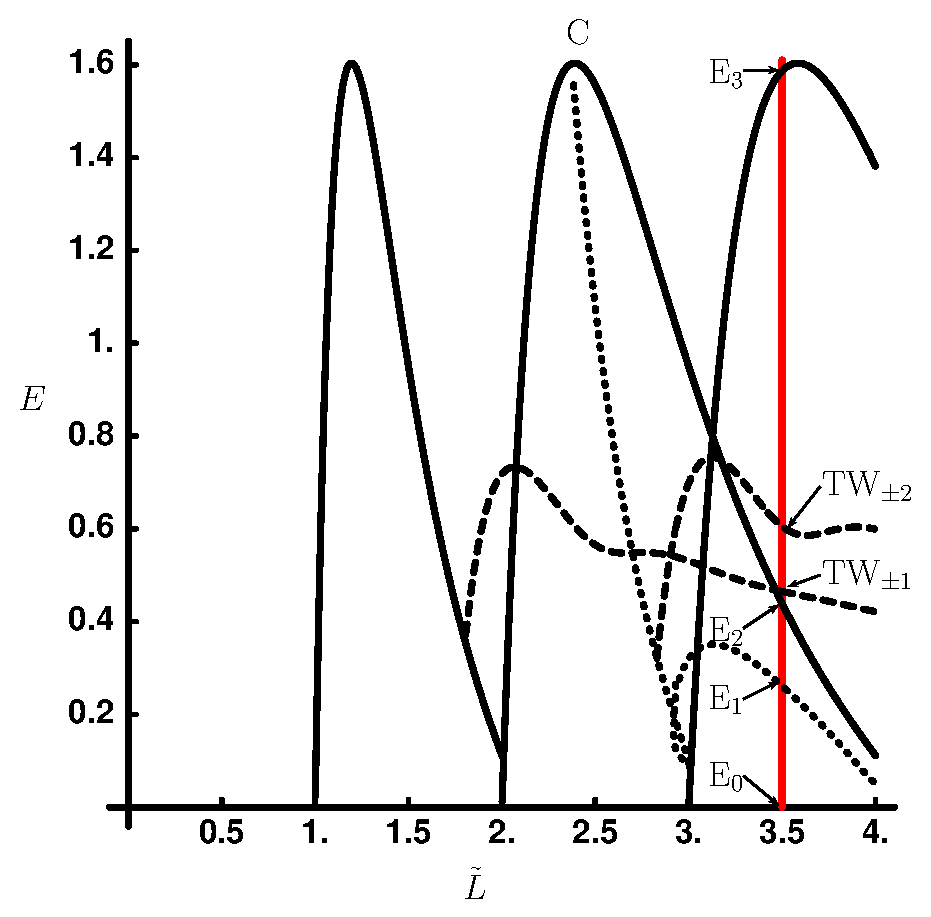
\includegraphics[width=0.5\textwidth]{ksBifDiag}
\end{center}
\caption[Bifurcation diagram for equilibria of Kuramoto-Sivashinsky eq.]
    {
    Bifurcation diagram for \eqva\ and \reqva\ of \KS\ system.
    Shown is the 2c to GLMRT bifurcation and the GLMRT to $\REQV{\pm}{2}$ bifurcation,
    points C and M in \rf{ksgreene88} respectively. The \reqv\ branch
    is followed up to our system size.
        }
\end{figure}
%%%%%%%%%%%%%%%%%%%%%%%%%%%%%%%%%%%%%%%%%%%%%%%%%%%%%%%%%%%%%%%%%%

\paragraph{Back in the saddle again:}
%
Kevrekidis, Nicolaenko and Scovel\rf{KNSks90} study \KS\ system
steady state bifurcations and the role of symmetry in the
existence of structurally stable (relative) homoclinic and
heteroclinic cycles between unstable saddles. The form  of
the equation they use is essentially that of Greene and Kim but
with bifurcation parameter connected to our by
$\alpha=4\tilde{L}^2$.


They prove that the bifurcation of the trivial state $y=0$ to
an $N$-cell state is a pitchfork. They observe that when the
$1$-cell state losses stability at point $A$ the eigenvector
corresponding to the zero eigenvalue of the {\stabmat}
aligns itself with the direction of uniform translation of the
system which, due to the translational invariance of \KSe\,
also corresponds to a zero eigenvalue. Thus the algebraic
multiplicity of the zero eigenvalue is $2$ while its geometric
multiplicity is $1$. Using this fact and a local,
$O(2)$-equivariant, approximation to the center manifold they
prove that this type of bifurcation creates traveling waves.

In typical numerical simulations  a trajectory initiated along
the (single) unstable eigendirection of an \eqv\ $y$ of
the $2$-cell branch would eventually become attracted to the
$L/4$-translated \eqv\ $y'$. Those (relative) homoclinic
connections
\ES{In \refref{KNSks90} the characterization homoclinic
connection is used. Here we prefer (to invent?) the term
relative homoclinic to emphasize the fact that the \eqva\
are symmetry related.}
although structurally unstable in most dynamical systems, were
found to be persistent in \KS\ system with the afore-mentioned
behavior observed in the range from $\tilde{L}\simeq 2.009$ up
to $\tilde{L}\simeq 2.375$  where the $2$-cell state becomes
stable. The existence and robustness of the saddle connection
was explained as follows\ES{The following may not make perfect
sense without reading the paper, especially the notation. I've
start re-writing \KS\ symmetries section to incorporate
information about the invariant subspaces which hopefully will
explain it but my progress is very slow.}:  The unstable
manifold of $y$ lies on an invariant subspace $L$ of \KS\ flow,
which is the fixed set of the isotropy subgroup of $O(2)$
defined by reflection with respect to imaginary axis. The
action of the generator of $D(4)$ (which sends y to y') on $L$
is to send it to the invariant subspace $R_{1}$ which is the
fixed set of $Z(2)$ defined by complex conjugation. The
converse is also true, i.e. the action of $D(4)$ sends $R_{1}$
to $L$. Thus the unstable eigendirection of $y$, lying on $L$,
is sent on $R_{1}$ for the $L/4$-shifted point $y'$. The two
invariant subspaces $L$ and $R_{1}$ are orthogonal and thus the
point $y'$ has only stable eigendirections on $L$ and appears
as a sink on that subspace. This explains why the (relative)
homoclinic connections are structurally stable in \KS\ system.

In the range $\tilde{L}=2.00$ when the $2$-cell branch comes to
existence with two unstable eigendirections, up to $\tilde{L}
\simeq 2.009$ when it merges to the $1$-cell branch and losses
one of its unstable eigendirections, a heteroclinic loop exists
that connects $2$-cell to $1$-cell solutions. The analysis is
similar to the previous case.

 An important remark in \refref{KNSks90} is that the exact
 saddle connections were observed using a numerical integrator
 based on an explicit Galerkin spectral discretization of \KSe,
 irrespective of how close to the \eqv\ along the unstable
 manifold we start. On the contrary, when an FFT-based
 integrator was used, trajectories with initial condition along
 the unstable direction of $y$ would approach the homoclinic
 connection but fly away along the direction of the unstable
 manifold of $y'$ and follow an approximate (relative)
 homoclinic loop. This is attributed to the Galerkin truncation
 respecting the symmetries and possessing the same subspaces as
 the original equation restricted to the first $n$ modes
 \ES{We
 observe the second kind of behavior and we both use an FFT
 based integrator. I plan to quickly write a Galerkin integrator
 and check to see if we get an exact connection.}.
    %
\ES{Here I discuss Brown and Kevrekidis\rf{BrKevr96} MTW.}
